\documentclass[a4paper]{report}
\usepackage[utf8]{inputenc}
\usepackage[portuguese]{babel}
\usepackage{indentfirst}
\usepackage{hyperref} % \href
\usepackage{graphicx} % \includegraphics
\usepackage{float}
\usepackage{caption}
\usepackage{subfig}
\usepackage[export]{adjustbox}
\usepackage{lscape}
\usepackage{geometry}

\hypersetup{pdftitle={Relatorio-DSS-parte2},
pdfauthor={Ariana Lousada, Carlos Gomes, Márcia Teixeira, Tiago Sousa},
colorlinks=true,
urlcolor=blue,
linkcolor=black}

\begin{document}

\title{Fase 2 \break
\large Grupo Nº 17}
\author{Ariana Lousada (A87998) \and Carlos Gomes (A77185) \and Márcia Teixeira (A80943) \and Tiago Sousa (A67674)}

\begin{center}
    \begin{minipage}{0.75\linewidth}
        \centering
        
\includegraphics[width=0.5\textwidth]{images/logo.png}\par\vspace{1cm}
        \vspace{1cm}
        \href{https://www.uminho.pt/}
        {\color{black}{\scshape\LARGE Universidade do Minho}}\par\vspace{1cm}
        \href{https://www.di.uminho.pt/}
        {\color{black}{\scshape\Large Departamento de Informática}} \par
        \maketitle
    \end{minipage}
\end{center}

\begin{figure}[H]
  \centering
  \begin{minipage}[b]{0.2\textwidth}
    \centering
    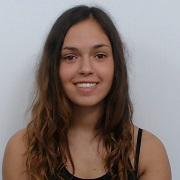
\includegraphics[width=\textwidth]{images/ariana.jpg}
    \caption*{Ariana Lousada (A87998)}
  \end{minipage}
  \hfill
  \begin{minipage}[b]{0.2\textwidth}
    \centering
    
\includegraphics[width=\textwidth]{images/carlos.png}
    \caption*{Carlos Gomes (A77815)}
  \end{minipage}
  \hfill
  \begin{minipage}[b]{0.2\textwidth}
    \centering
    
\includegraphics[width=\textwidth]{images/marcia.png}
    \caption*{Márcia Teixeira (A80943)}
  \end{minipage}
  \hfill
  \begin{minipage}[b]{0.2\textwidth}
    \centering
    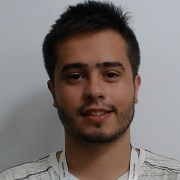
\includegraphics[width=\textwidth]{images/tiago.jpg}
    \caption*{Tiago Sousa (A67674)}
  \end{minipage}
  
\end{figure}

\tableofcontents

\pagebreak

\chapter{Introdução}
No âmbito da Unidade Curricular de Desenvolvimento de Sistemas de Software, foi-nos proposta a realização de um trabalho prático que visa a criação de um sistema de gestão de \textit{stocks} de um armazém de uma fábrica.

Com este relatório temos o objectivo de apresentar a modelação concetual do projeto da unidade curricular de Desenvolvimento de Sistemas de Software. Nesta segunda fase, iremos desenvolver um modelo concetual, com auxílio a diagramas de componentes, de sequência e de classes.\\

Para isto, foram propostos vários Use Cases pela equipa docente, com os quais vamos trabalhar ao longo desta fase do projeto.



\chapter{Diagrama de Componentes}
    De modo a sermos capazes de perceber e "dividir" as necessidades provenientes dos Use Cases apresentados primeiro temos de saber quantas componentes são necessárias e a importância de cada uma.
    
    Primeiramente, criámos uma \textit{User Interface} do \textit{Armazém} para permitir acesso às várias entidades que o necessitam. Para além disto, resolvemos inserir uma \textit{Data Layer} ao armazém, uma vez que vai ser este que vai conter a maior parte da informação.
    De seguida decidimos atribuir uma interface a cada um dos atores dos Use Cases propostos (uma vez que todos interagem com o sistema do armazém de alguma forma, através de vários métodos) adicionando mais uma, a \textit{ISSEncarregado}, uma vez que no contexto do nosso projeto é a entidade \textbf{Encarregado} que interage com o \textbf{Servidor de Produção}, o que foi estabalecido na primeira fase deste projeto.\footnote{Para ver o diagrama de componentes desenvolvido, consultar apêndice A}
    


\chapter{Diagrama de Classes}
    Para analisarmos melhor os Use Cases propostos, é necessário ver como o sistema se deve comportar com cada um destes, isto é, as suas responsabilidades: o que deve ser capaz de fazer, face a sua utilização. Para isto, é necessário detetar as responsabilidades do sistema em cada Use Case e traduzi-las para uma API da lógica de negócio, que suporte o Use Case associado.\footnote{Para analisar os Use Cases com maior detalhe, consultar o documento Excel UseCases.xlsx anexado juntamente com este relatório.}
    
    Para isto, criámos uma classe para cada ator referido: Gestor, Leitor de códigos QR, Robot e Servidor de Produção. Para além disto, adicionámos uma classe Armazém, que contém o inventário (Lista de produtos que estão armazenados no seu espaço físico) e a informação a cerca dos utilizadores que têm acesso (Lista de credencias), três diferentes classes que simbolizam objetos utilizados para representar diferentes dados necessários (OrdTransp, CodQR, Localizacao e Palete) e uma classe Encarregado, pela qual o Armazém interage com o Servidor de Produção, uma classe semelhante ao Gestor, apenas com diferentes funções.\footnote{Para analisar o Diagrama de Classes com maior detalhe, consultar o apêndice B}


\chapter{Diagramas de Sequência}
    De modo a melhorar a organização, foi necessário desenvolver um diagrama de sequência para cada Use case.
    
    \begin{enumerate}
       
    
    
        \item \textbf{Use Case - Consultar listagem de localizações}
            
            Para este Use Case, considerámos que o Gestor interage com o sistema através de uma interface de estrutura semelhante ao multibanco, no qual cada ação é reresentada por um número. A função apresentada \textit{executarAcao} é a que interpreta a escolha do utilizador. Neste caso, a opção vai estar relacionada com a listagem de localizações do armazém, que é pedida ao sistema. Caso não existam produtos, o sistema não devolve nada.
            
        \begin{figure}[H]
        \centering
        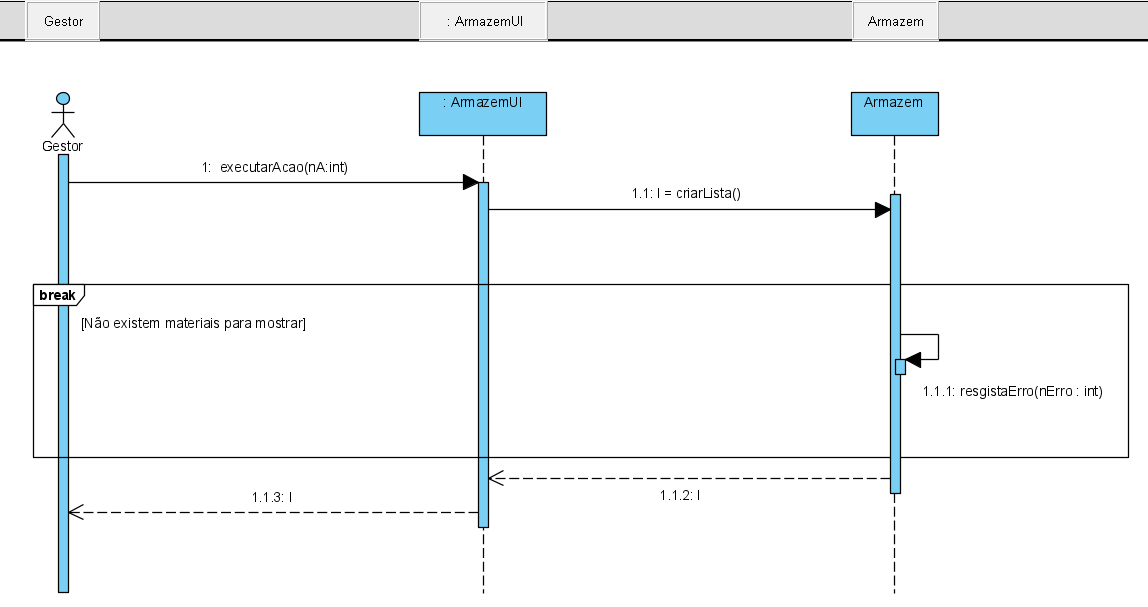
\includegraphics[scale=0.50]{images/UC-ConsultarListagem.PNG}
        \caption{}
        \end{figure}
        
       \pagebreak 
       \item \textbf{Use Case - Iniciar sessão}
            
            Neste caso, o sistema testa as credenciais inseridas pelo utilizador. Se forem válidas, permite acesso; caso contrário, são solicitadas novas credenciais, informando o utilizador que as inseridas não existem.
       
       \begin{figure}[H]
        \centering
        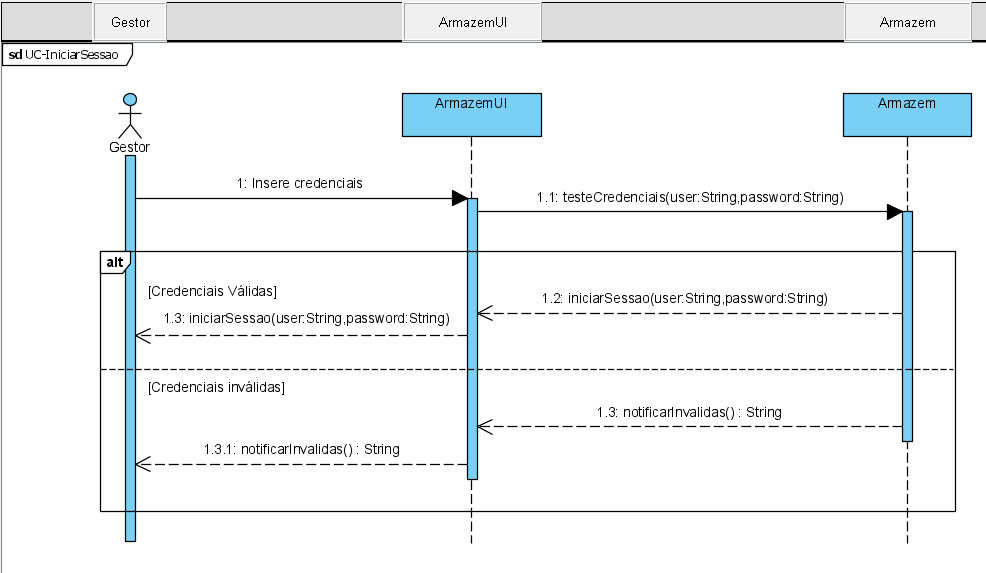
\includegraphics[scale=0.50]{images/UC-IniciarSessao.PNG}
        \caption{}
        \end{figure}
       
       
       \item \textbf{Use Case - Terminar sessão}
       
       \begin{figure}[H]
        \centering
        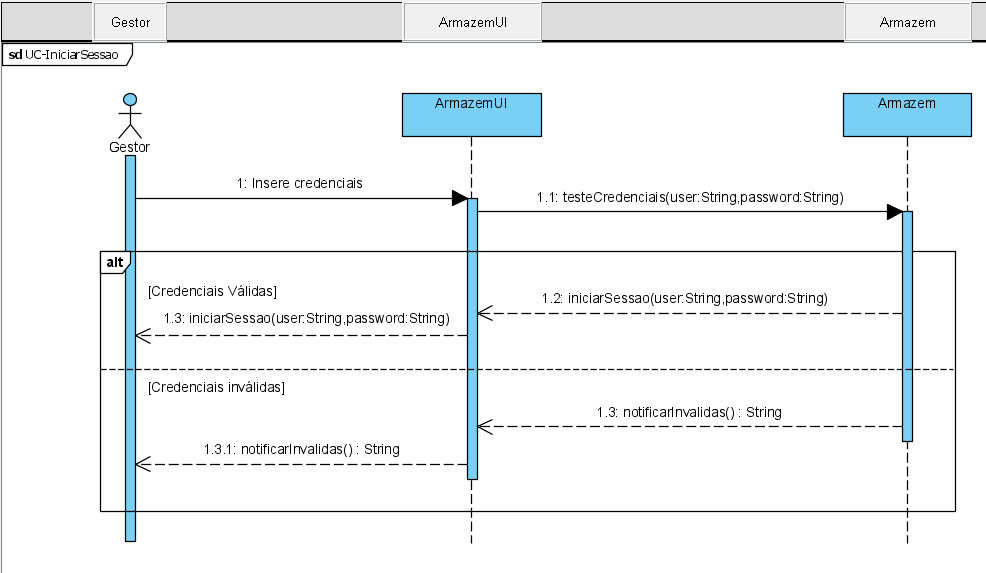
\includegraphics[scale=0.50]{images/UC-IniciarSessao.PNG}
        \caption{}
        \end{figure}
       
       \pagebreak
       \item \textbf{Use Case - Comunicar código QR}
            
            Neste caso, o leitor de códigos QR vai fazer a leitura deste e posteriormente enviá-lo para o sistema. Se algum erro ocorrer, o sistema regista esse erro e pede novamente o código ao mesmo leitor.
       
        \begin{figure}[H]
        \centering
        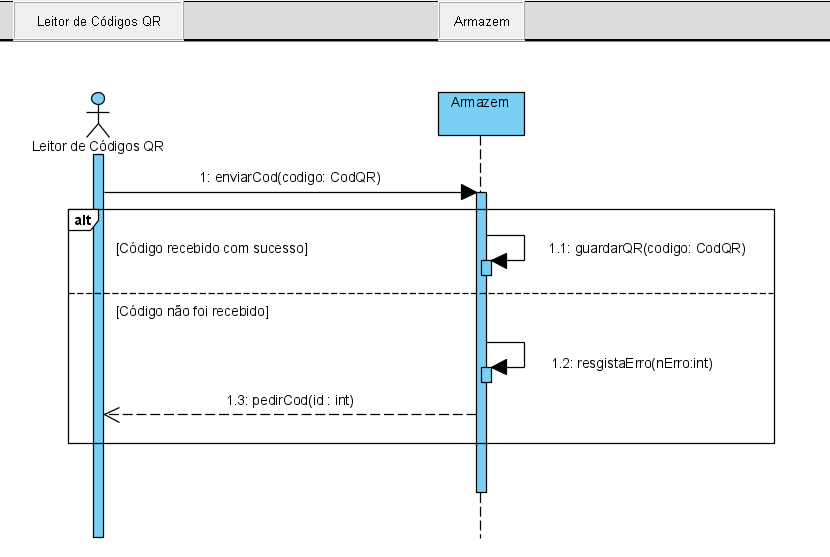
\includegraphics[scale=0.50]{images/UC-ComunicarQR.PNG}
        \caption{}
        \end{figure}
        
        \item \textbf{Use Case - Sistema comunica ordem de transporte}
            
            Neste Use Case o sistema constroi Ordens de Transporte(constituidas pelo local de entrega/recolha e pelo identificador do robot) e envia aos seus diferentes robots de modo a executar entregas e recolhas de Paletes. Caso ocorra um erro no envio da ordem de transporte, o sitema regista o erro e tenta novamente enviá-la.
            
            \begin{figure}[H]
             \centering
             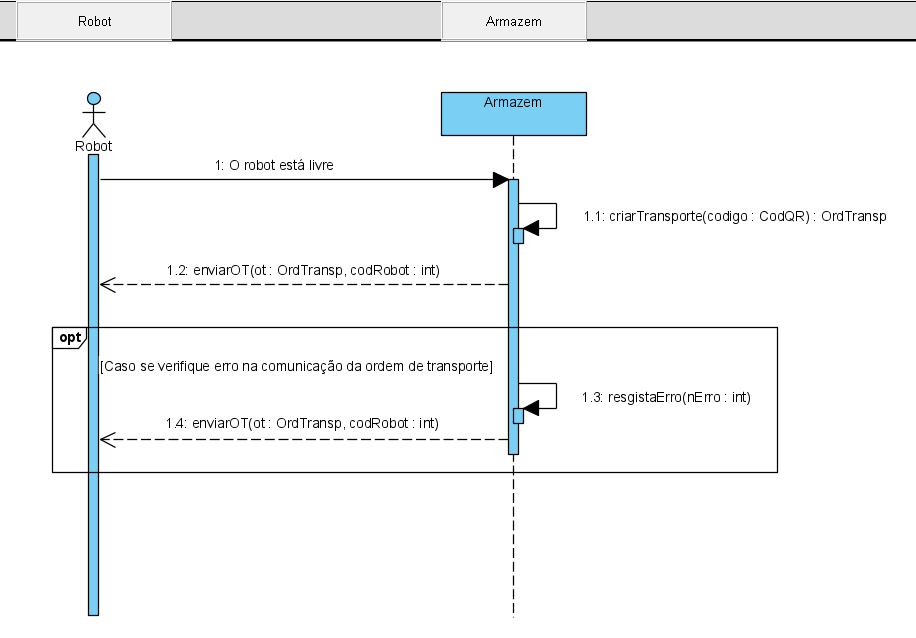
\includegraphics[scale=0.50]{images/UC-ComunicaOT.PNG}
             \caption{}
            \end{figure}
        
        \pagebreak
        \item \textbf{Use Case - Notificar recolha de paletes}
            
            \begin{figure}[H]
             \centering
             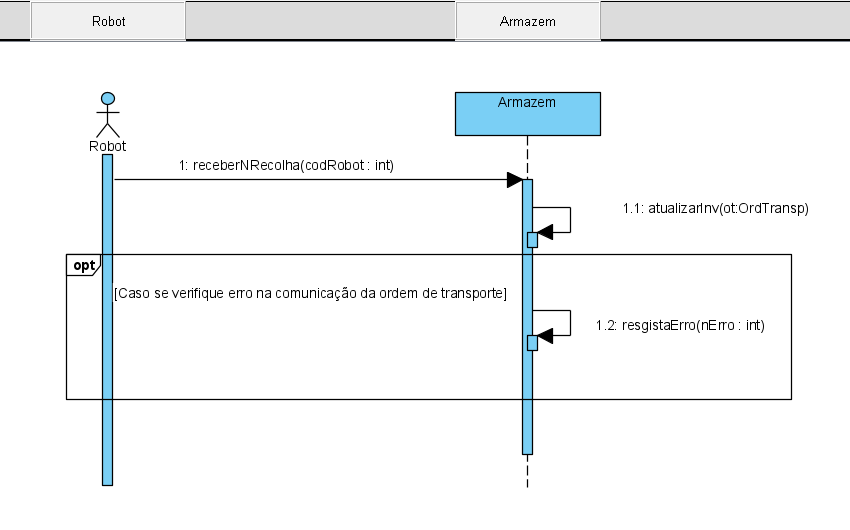
\includegraphics[scale=0.50]{images/UC-NRecolha.PNG}
             \caption{}
            \end{figure}
        
        \item \textbf{Use Case - Notificar entrega de paletes}
            
            \begin{figure}[H]
             \centering
             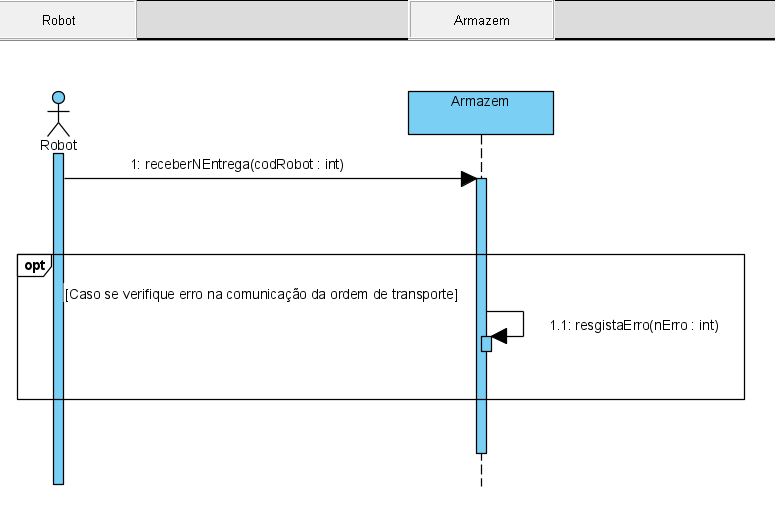
\includegraphics[scale=0.50]{images/UC-NEntrega.PNG}
             \caption{}
            \end{figure}    
        
        \pagebreak
        \item \textbf{Use Case - Requisitar paletes}
            
            Neste Use Case, o Servidor de Produção solicita uma requisição ao Armazém. De seguida, este vai verificar a disponibilidade de cada palete pedida no seu inventário. Se todas as paletes pedidas estiverem disponíveis, o Encarregado confirma a requisição e esta é efetuada (sendo que o encarregado também pode recusar a requisição). Caso existam paletes indisponíveis, é lhe dada a escolha ao servidor de proceder com a requisição (encomendar apenas as paletes disponíveis) ou cancelar. 
            
            \begin{figure}[H]
             \centering
             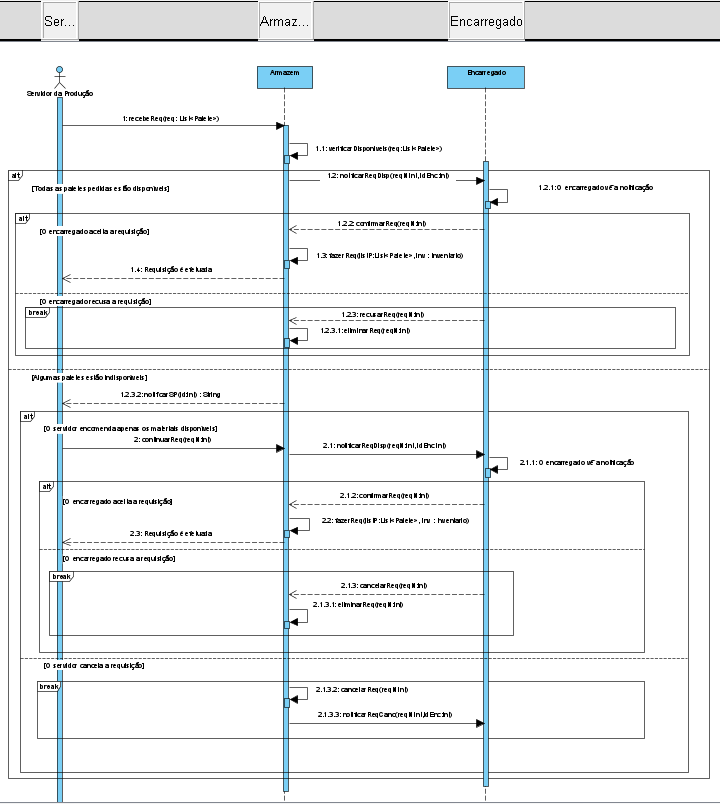
\includegraphics[scale=0.90]{images/UC-Requisicao.PNG}
             \caption{}
            \end{figure}   
        
       
    \end{enumerate}

\chapter{Conclusão - DSS}
Através da realização desta segunda etapa do trabalho conseguimos ver que é mais fácil organizar um determinado projeto com o tipo de modelagem utilizado .\\ 

Este planeamento e modelação permite-nos separar melhor as responsabilidades de cada entidade no projeto, o que resulta numa melhor organização e maior facilidade de interpretação.\\

%Resumidamente, com este projeto (tal como lecionado nas aula desta Unidade Curricular), fomos capazes de:
        \begin{itemize} \par
            \item Dividir fluxos em sequências de transações (com os diagramas de sequência).
            \item Identificar responsabilidades da lógica de negócio (com a descrição dos Use Cases propostos).
            \item Identificar métodos e organizá-los entre as diferentes entidades (com o diagrama de classes).
            \item Agrupar os métodos em sub-sistemas (com o diagrama de componentes).
        \end{itemize}
    
    
\appendix
    \chapter{Diagrama de Componentes}
        \begin{figure}[H]
            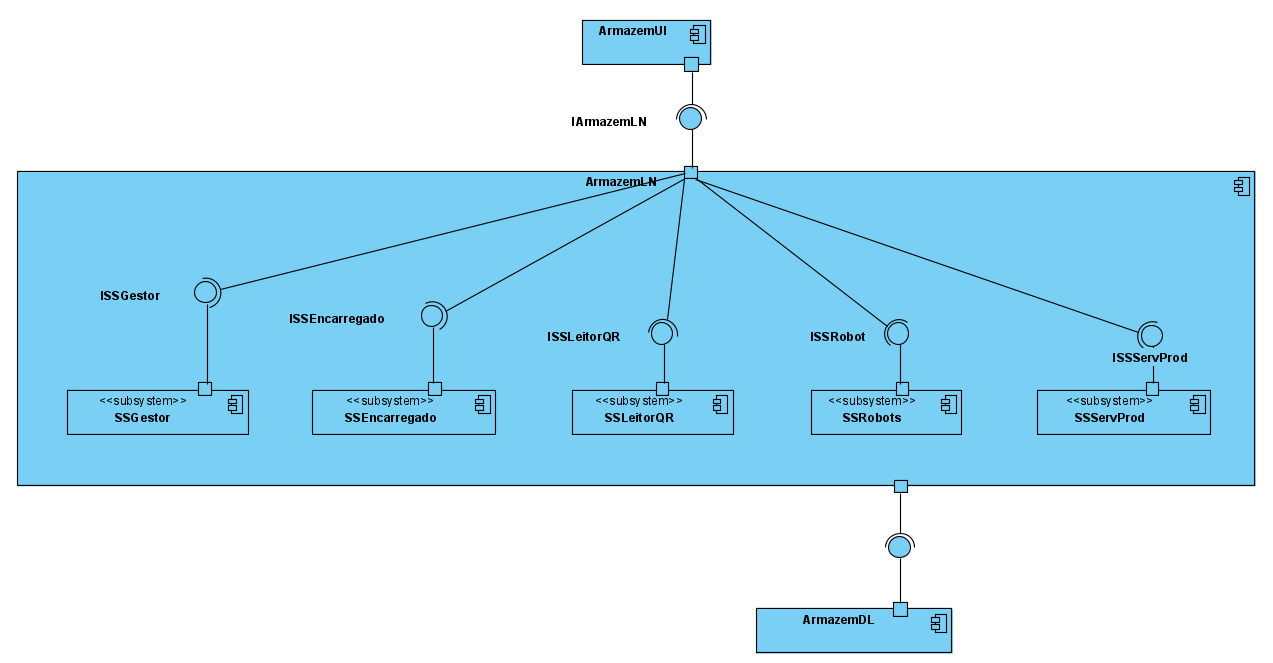
\includegraphics[scale=0.40, center]{images/componentDiagram.png}
            \caption{}
        \end{figure}

    \chapter{Diagrama de Classes}
        \begin{figure}[H]
            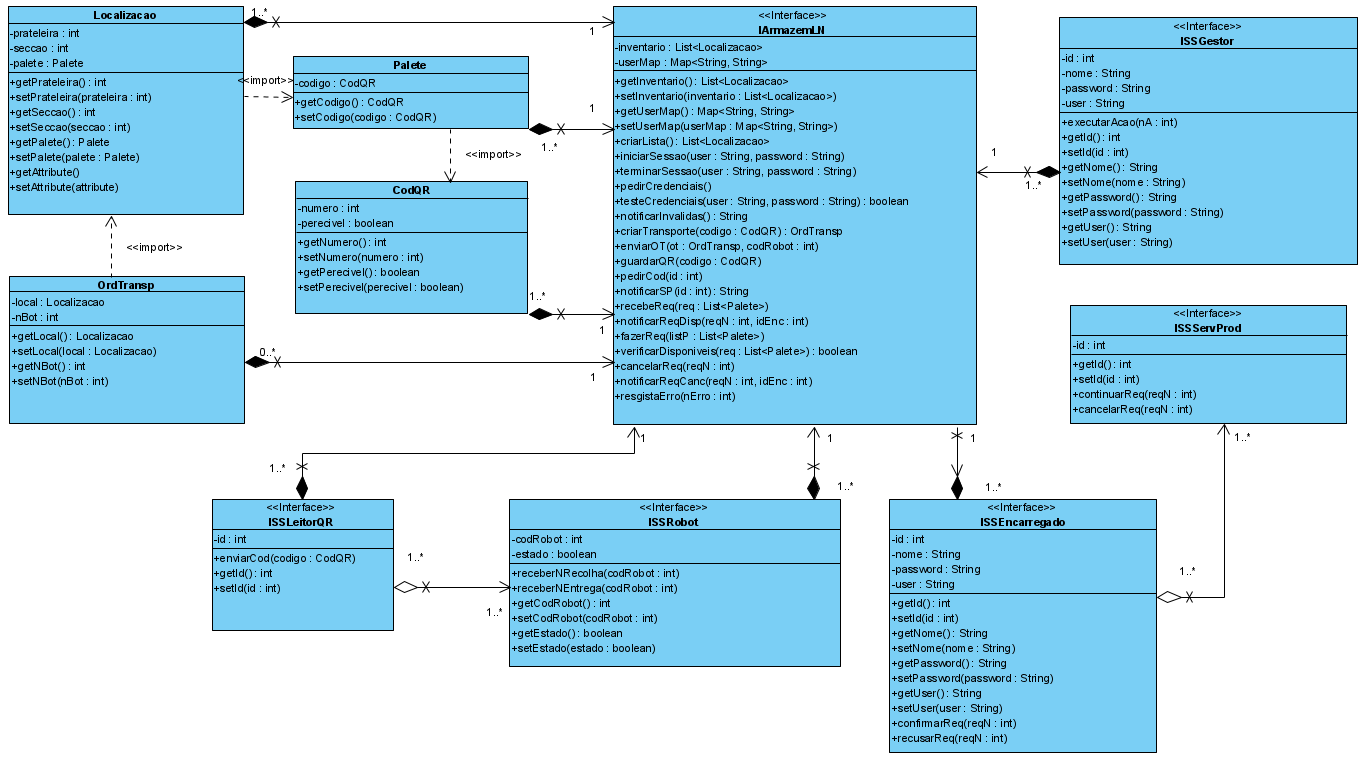
\includegraphics[scale=0.60, center]{images/ClassDiagram.png}
            \caption{}
        \end{figure}

\end{document}